\documentclass{standalone}
\usepackage{tikz}
\usetikzlibrary{patterns, positioning}
\usepackage[sfdefault]{ClearSans} %% option 'sfdefault' activates Clear Sans as the default text font
\usepackage[T1]{fontenc}

\begin{document}
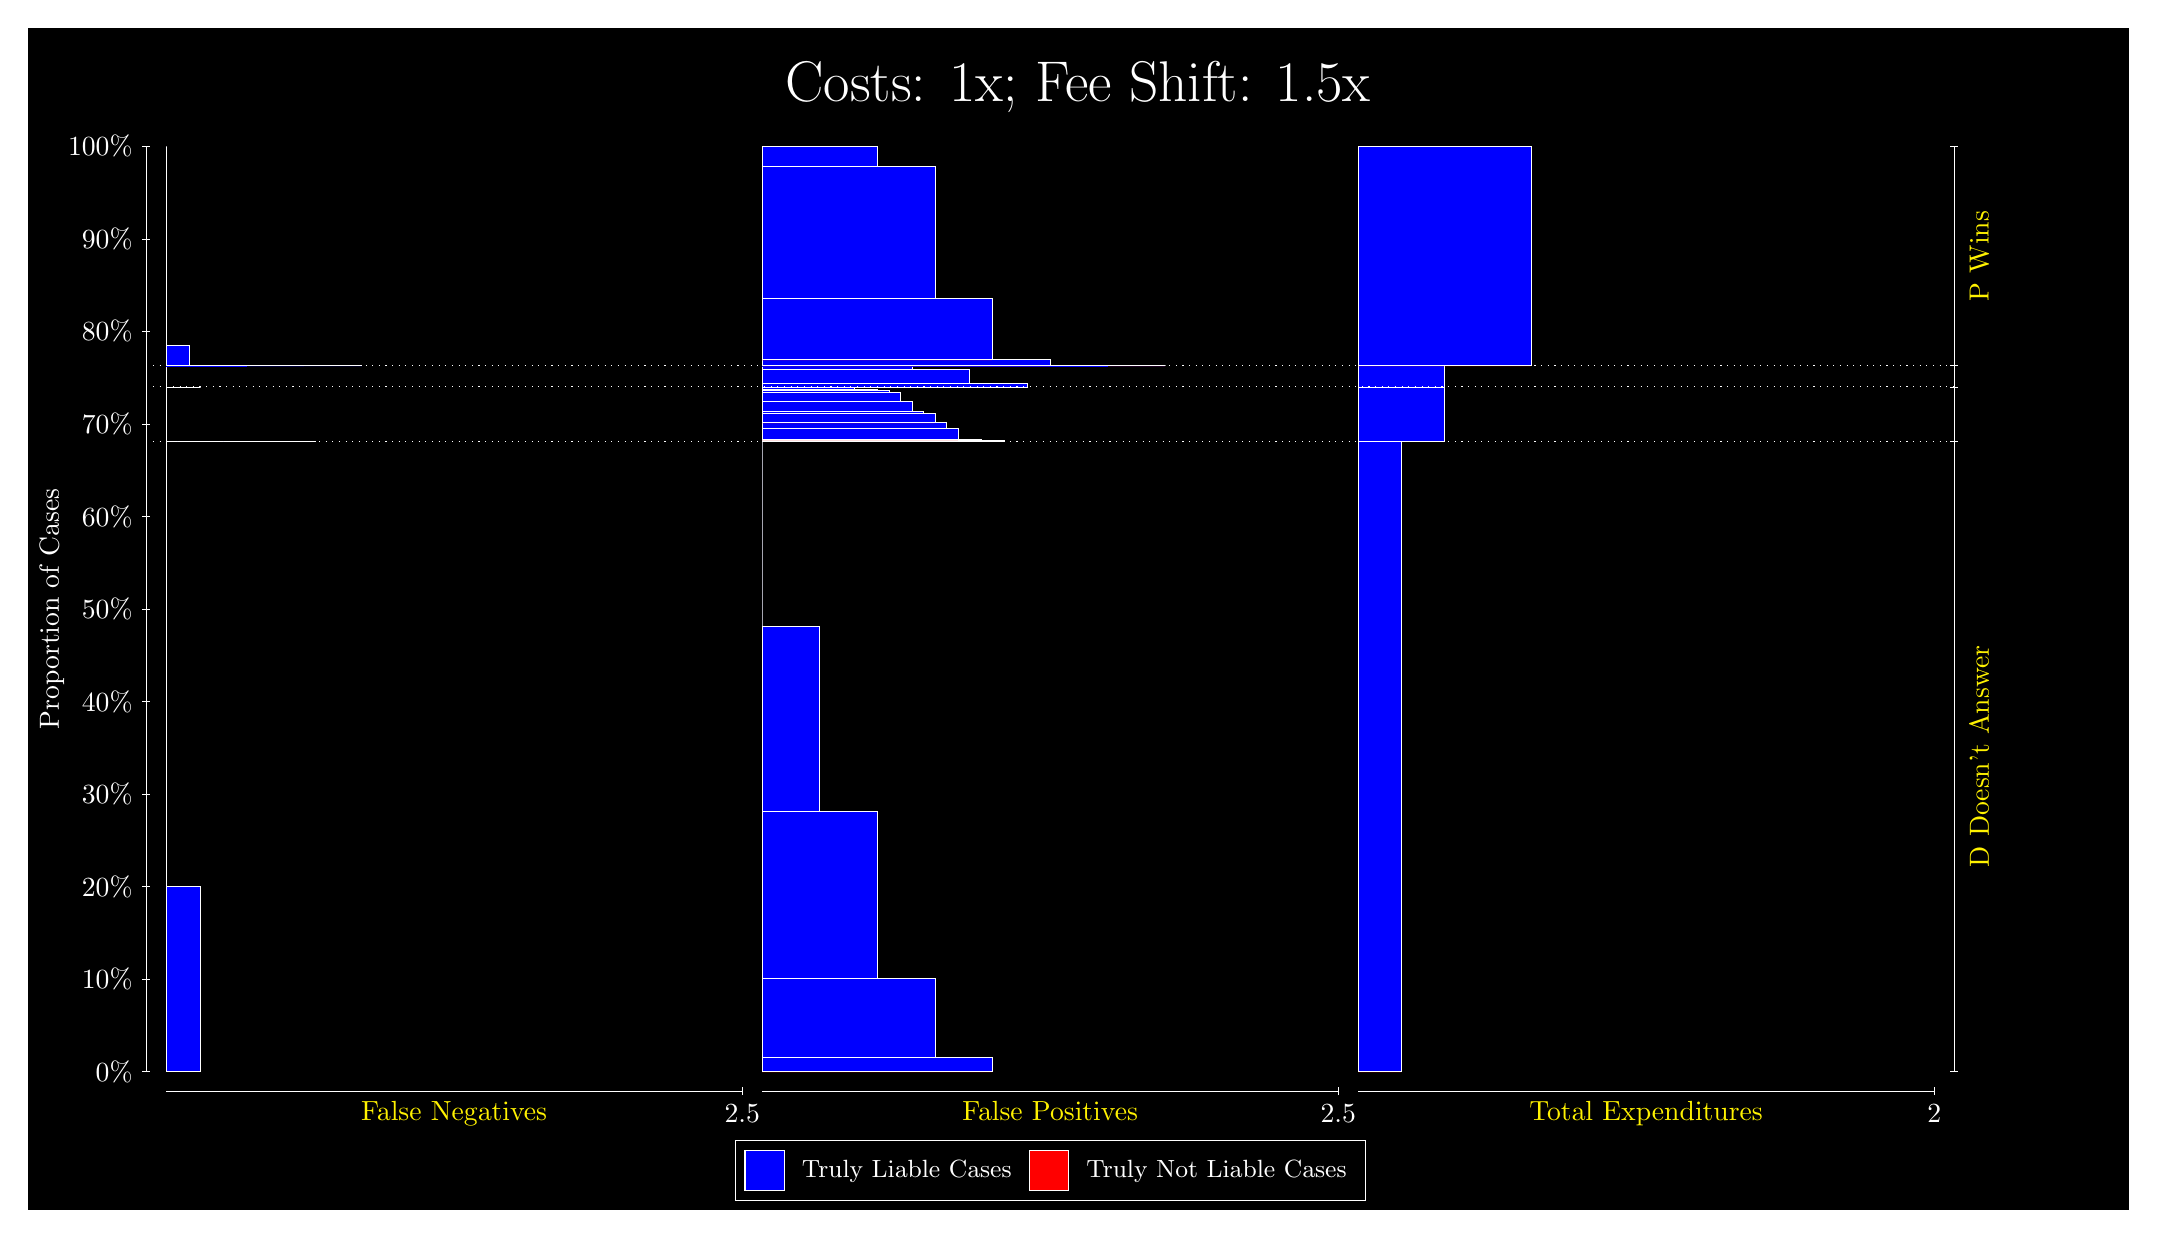
\begin{tikzpicture}
\draw[fill=black] (0,0) rectangle (26.667,15);
\draw[text=white] (0,13.5) rectangle (26.667,15) node[midway] {\huge Costs: 1x; Fee Shift: 1.5x};
\draw[white, very thin] (1.5,1.75) -- (1.5,13.5);
\node[rotate=90, text=white, anchor=center] at (0.3, 7.625) {Proportion of Cases};
\draw[white, very thin] (1.45,1.75) -- (1.55,1.75);
\node[text=white, anchor=east] at (1.45, 1.75) {0\%};
\draw[white, very thin] (1.45,2.925) -- (1.55,2.925);
\node[text=white, anchor=east] at (1.45, 2.925) {10\%};
\draw[white, very thin] (1.45,4.1) -- (1.55,4.1);
\node[text=white, anchor=east] at (1.45, 4.1) {20\%};
\draw[white, very thin] (1.45,5.275) -- (1.55,5.275);
\node[text=white, anchor=east] at (1.45, 5.275) {30\%};
\draw[white, very thin] (1.45,6.45) -- (1.55,6.45);
\node[text=white, anchor=east] at (1.45, 6.45) {40\%};
\draw[white, very thin] (1.45,7.625) -- (1.55,7.625);
\node[text=white, anchor=east] at (1.45, 7.625) {50\%};
\draw[white, very thin] (1.45,8.8) -- (1.55,8.8);
\node[text=white, anchor=east] at (1.45, 8.8) {60\%};
\draw[white, very thin] (1.45,9.975) -- (1.55,9.975);
\node[text=white, anchor=east] at (1.45, 9.975) {70\%};
\draw[white, very thin] (1.45,11.15) -- (1.55,11.15);
\node[text=white, anchor=east] at (1.45, 11.15) {80\%};
\draw[white, very thin] (1.45,12.325) -- (1.55,12.325);
\node[text=white, anchor=east] at (1.45, 12.325) {90\%};
\draw[white, very thin] (1.45,13.5) -- (1.55,13.5);
\node[text=white, anchor=east] at (1.45, 13.5) {100\%};

\draw[white, very thin] (24.457,1.75) -- (24.457,13.5);
\draw[white, very thin] (24.407,1.75) -- (24.507,1.75);
\node[anchor=west] at (24.407, 1.75) {};
\draw[white, very thin] (24.407,9.7533) -- (24.507,9.7533);
\node[anchor=west] at (24.407, 9.7533) {};
\draw[white, very thin] (24.407,10.446) -- (24.507,10.446);
\node[anchor=west] at (24.407, 10.446) {};
\draw[white, very thin] (24.407,10.713) -- (24.507,10.713);
\node[anchor=west] at (24.407, 10.713) {};
\draw[white, very thin] (24.407,13.5) -- (24.507,13.5);
\node[anchor=west] at (24.407, 13.5) {};

\draw[white, very thin, fill=blue] (1.75,1.75) rectangle (2.1891,4.0999);
\draw[white, very thin, fill=red] (1.75,4.0999) rectangle (1.75,4.0999);
\draw[white, very thin, fill=blue] (1.75,4.0999) rectangle (1.75,9.7533);
\draw[white, very thin, fill=blue] (1.75,9.7533) rectangle (3.6529,9.7533);
\draw[white, very thin, fill=blue] (1.75,9.7533) rectangle (3.3602,9.7533);
\draw[white, very thin, fill=blue] (1.75,9.7533) rectangle (3.0674,9.7533);
\draw[white, very thin, fill=blue] (1.75,9.7533) rectangle (2.921,9.7533);
\draw[white, very thin, fill=blue] (1.75,9.7533) rectangle (2.7746,9.7533);
\draw[white, very thin, fill=blue] (1.75,9.7533) rectangle (2.6283,9.7533);
\draw[white, very thin, fill=blue] (1.75,9.7533) rectangle (2.4819,9.7533);
\draw[white, very thin, fill=blue] (1.75,9.7533) rectangle (2.3355,9.7533);
\draw[white, very thin, fill=blue] (1.75,9.7533) rectangle (2.1891,9.7534);
\draw[white, very thin, fill=blue] (1.75,9.7534) rectangle (2.0428,9.7534);
\draw[white, very thin, fill=blue] (1.75,9.7534) rectangle (1.8964,9.7534);
\draw[white, very thin, fill=red] (1.75,9.7534) rectangle (1.75,9.7534);
\draw[white, very thin, fill=blue] (1.75,9.7534) rectangle (1.75,10.446);
\draw[white, very thin, fill=blue] (1.75,10.446) rectangle (2.1891,10.446);
\draw[white, very thin, fill=red] (1.75,10.446) rectangle (1.75,10.446);
\draw[white, very thin, fill=blue] (1.75,10.446) rectangle (1.75,10.713);
\draw[white, very thin, fill=blue] (1.75,10.713) rectangle (4.2384,10.713);
\draw[white, very thin, fill=blue] (1.75,10.713) rectangle (3.5065,10.713);
\draw[white, very thin, fill=blue] (1.75,10.713) rectangle (2.7746,10.713);
\draw[white, very thin, fill=blue] (1.75,10.713) rectangle (2.7746,10.716);
\draw[white, very thin, fill=blue] (1.75,10.716) rectangle (2.0428,10.717);
\draw[white, very thin, fill=blue] (1.75,10.717) rectangle (2.0428,10.967);
\draw[white, very thin, fill=red] (1.75,10.967) rectangle (1.75,10.967);
\draw[white, very thin, fill=blue] (1.75,10.967) rectangle (1.75,13.5);
\draw[white, very thin, fill=red] (9.3189,1.75) rectangle (12.246,1.75);
\draw[white, very thin, fill=blue] (9.3189,1.75) rectangle (12.246,1.9268);
\draw[white, very thin, fill=blue] (9.3189,1.9268) rectangle (11.515,2.9326);
\draw[white, very thin, fill=blue] (9.3189,2.9326) rectangle (10.783,5.0553);
\draw[white, very thin, fill=blue] (9.3189,5.0553) rectangle (10.051,7.4034);
\draw[white, very thin, fill=blue] (9.3189,7.4034) rectangle (9.3189,9.7533);
\draw[white, very thin, fill=red] (9.3189,9.7533) rectangle (12.393,9.7533);
\draw[white, very thin, fill=blue] (9.3189,9.7533) rectangle (12.393,9.767);
\draw[white, very thin, fill=red] (9.3189,9.767) rectangle (12.1,9.767);
\draw[white, very thin, fill=blue] (9.3189,9.767) rectangle (12.1,9.7746);
\draw[white, very thin, fill=red] (9.3189,9.7746) rectangle (11.807,9.7746);
\draw[white, very thin, fill=blue] (9.3189,9.7746) rectangle (11.807,9.9191);
\draw[white, very thin, fill=blue] (9.3189,9.9191) rectangle (11.661,9.9899);
\draw[white, very thin, fill=red] (9.3189,9.9899) rectangle (11.515,9.9899);
\draw[white, very thin, fill=blue] (9.3189,9.9899) rectangle (11.515,10.109);
\draw[white, very thin, fill=blue] (9.3189,10.109) rectangle (11.368,10.135);
\draw[white, very thin, fill=red] (9.3189,10.135) rectangle (11.222,10.135);
\draw[white, very thin, fill=blue] (9.3189,10.135) rectangle (11.222,10.266);
\draw[white, very thin, fill=blue] (9.3189,10.266) rectangle (11.075,10.377);
\draw[white, very thin, fill=blue] (9.3189,10.377) rectangle (10.929,10.398);
\draw[white, very thin, fill=blue] (9.3189,10.398) rectangle (10.783,10.416);
\draw[white, very thin, fill=blue] (9.3189,10.416) rectangle (10.636,10.419);
\draw[white, very thin, fill=blue] (9.3189,10.419) rectangle (10.49,10.437);
\draw[white, very thin, fill=blue] (9.3189,10.437) rectangle (10.344,10.446);
\draw[white, very thin, fill=blue] (9.3189,10.446) rectangle (10.197,10.446);
\draw[white, very thin, fill=blue] (9.3189,10.446) rectangle (10.051,10.446);
\draw[white, very thin, fill=blue] (9.3189,10.446) rectangle (9.9044,10.446);
\draw[white, very thin, fill=blue] (9.3189,10.446) rectangle (9.758,10.446);
\draw[white, very thin, fill=blue] (9.3189,10.446) rectangle (9.6116,10.446);
\draw[white, very thin, fill=blue] (9.3189,10.446) rectangle (9.4652,10.446);
\draw[white, very thin, fill=blue] (9.3189,10.446) rectangle (9.3189,10.446);
\draw[white, very thin, fill=red] (9.3189,10.446) rectangle (12.686,10.446);
\draw[white, very thin, fill=blue] (9.3189,10.446) rectangle (12.686,10.488);
\draw[white, very thin, fill=blue] (9.3189,10.488) rectangle (11.954,10.666);
\draw[white, very thin, fill=blue] (9.3189,10.666) rectangle (11.222,10.712);
\draw[white, very thin, fill=blue] (9.3189,10.712) rectangle (10.49,10.713);
\draw[white, very thin, fill=blue] (9.3189,10.713) rectangle (9.758,10.713);
\draw[white, very thin, fill=red] (9.3189,10.713) rectangle (14.442,10.713);
\draw[white, very thin, fill=blue] (9.3189,10.713) rectangle (14.442,10.713);
\draw[white, very thin, fill=red] (9.3189,10.713) rectangle (13.71,10.713);
\draw[white, very thin, fill=blue] (9.3189,10.713) rectangle (13.71,10.714);
\draw[white, very thin, fill=red] (9.3189,10.714) rectangle (12.978,10.714);
\draw[white, very thin, fill=blue] (9.3189,10.714) rectangle (12.978,10.79);
\draw[white, very thin, fill=red] (9.3189,10.79) rectangle (12.246,10.79);
\draw[white, very thin, fill=blue] (9.3189,10.79) rectangle (12.246,11.568);
\draw[white, very thin, fill=red] (9.3189,11.568) rectangle (11.515,11.568);
\draw[white, very thin, fill=blue] (9.3189,11.568) rectangle (11.515,13.246);
\draw[white, very thin, fill=blue] (9.3189,13.246) rectangle (10.783,13.497);
\draw[white, very thin, fill=blue] (9.3189,13.497) rectangle (10.051,13.5);
\draw[white, very thin, fill=blue] (9.3189,13.5) rectangle (9.3189,13.5);
\draw[white, very thin, fill=red] (16.888,1.75) rectangle (17.437,1.75);
\draw[white, very thin, fill=blue] (16.888,1.75) rectangle (17.437,9.7533);
\draw[white, very thin, fill=red] (16.888,9.7533) rectangle (17.986,9.7533);
\draw[white, very thin, fill=blue] (16.888,9.7533) rectangle (17.986,10.446);
\draw[white, very thin, fill=red] (16.888,10.446) rectangle (17.986,10.446);
\draw[white, very thin, fill=blue] (16.888,10.446) rectangle (17.986,10.713);
\draw[white, very thin, fill=red] (16.888,10.713) rectangle (19.083,10.713);
\draw[white, very thin, fill=blue] (16.888,10.713) rectangle (19.083,13.5);
\draw[white, dotted] (1.5,9.7533) -- (24.457,9.7533);
\draw[white, dotted] (1.5,10.446) -- (24.457,10.446);
\draw[white, dotted] (1.5,10.713) -- (24.457,10.713);
\draw[white, very thin] (1.75,1.5) -- (9.0689,1.5);
\node[text=yellow, anchor=north] at (5.4094, 1.5) {False Negatives};
\draw[white, very thin] (9.0689,1.45) -- (9.0689,1.55);
\node[text=white, anchor=north] at (9.0689, 1.45) {2.5};

\draw[white, very thin] (9.3189,1.5) -- (16.638,1.5);
\node[text=yellow, anchor=north] at (12.978, 1.5) {False Positives};
\draw[white, very thin] (16.638,1.45) -- (16.638,1.55);
\node[text=white, anchor=north] at (16.638, 1.45) {2.5};

\draw[white, very thin] (16.888,1.5) -- (24.207,1.5);
\node[text=yellow, anchor=north] at (20.547, 1.5) {Total Expenditures};
\draw[white, very thin] (24.207,1.45) -- (24.207,1.55);
\node[text=white, anchor=north] at (24.207, 1.45) {2};

\node[text=yellow, centered, rotate=90] at (24.777, 5.7517) {D Doesn't Answer};


\node[text=yellow, centered, rotate=90] at (24.777, 12.106) {P Wins};

\draw (12.978300999999998,1.5) node[draw=none] (baseCoordinate) {};
\begin{scope}[align=center]
        \matrix[scale=0.5, draw=white, below=0.5cm of baseCoordinate, nodes={draw}, column sep=0.1cm]{
            \node[rectangle, draw, minimum width=0.5cm, minimum height=0.5cm, fill=blue] {}; &
            \node[draw=none, font=\small, text=white] (B) {Truly Liable Cases}; &
            \node[rectangle, draw, minimum width=0.5cm, minimum height=0.5cm, fill=red] {}; &
            \node[draw=none, font=\small, text=white] (B) {Truly Not Liable Cases}; \\
            };
\end{scope}

\end{tikzpicture}
\end{document}